%====================================================
% ----                   Cap 4
%====================================================
\renewcommand{\caminhograficos}{aulas/cap_4/graficos}
\newcommand{\figDa}{
    \begin{figure}[H]
        \centering
        \includegraphics[width=0.8\textwidth]{fig-4.1.png}
        \caption{A figura representa o efeito  da aceleração perante a velocidade num movimento acelerado.}        
        \label{fig:mruv_acel_vec}
    \end{figure}
}

\newcommand{\figDb}{
    \centering
    \includegraphics[width=\textwidth]{fig-4.2.png}
    \begin{minipage}{0.65\textwidth}
        \captionsetup{hypcap=false}
        \captionof{figure}{Representação esquemática de uma colisão de uma bala na madeira.}
        \label{fig:bala_tabua}
    \end{minipage}
}
% --- DEDUÇÃO DA POSIÇÃO NO MRUV ---
\newcommand{\deducaoPosicaoMRUV}{
    \begin{example}
        A dedução desta função pode ser feita através da área sob o gráfico $v \times t$. No MRUV, a área entre o \cref{fig:grafico_area_mruv} e o eixo do tempo corresponde ao deslocamento $\Delta s$. 

        Considerando o gráfico de uma reta inclinada (trapézio), a área é:
        \[ \text{Área} = \frac{(B + b) \cdot h}{2} \implies \Delta s = \frac{(v + v_0) \cdot t}{2} \]
        Substituindo $v = v_0 + at$:
        \[ s - s_0 = \frac{(v_0 + at + v_0) \cdot t}{2} \]
        \[ s - s_0 = v_0t + \frac{1}{2}at^2 \implies s = s_0 + v_0t + \frac{1}{2}at^2 \]
    \end{example}
}

\newcommand{\deducaoTorricelli}{
    \subsection{Dedução Matemática}

    Para deduzir a equação, combinamos a Função Horária da Velocidade com a Função Horária da Posição através da eliminação do parâmetro $t$.

    \begin{enumerate}
        \item Isolamos o tempo ($t$) na Função Horária da Velocidade:
        \begin{equation}
            v = v_0 + at \implies t = \frac{v - v_0}{a}
        \end{equation}

        \item Substituímos a expressão de $t$ na Função Horária da Posição ($\Delta s = v_0 t + \frac{1}{2}at^2$):
        \begin{equation}
            \Delta s = v_0 \left( \frac{v - v_0}{a} \right) + \frac{1}{2}a \left( \frac{v - v_0}{a} \right)^2
        \end{equation}

        \item Desenvolvemos o produto notável e distribuímos os termos:
        \begin{equation}
            \Delta s = \frac{v_0 v - v_0^2}{a} + \frac{a(v^2 - 2v v_0 + v_0^2)}{2a^2}
        \end{equation}

        \item Simplificamos o termo $a$ e reduzimos ao mesmo denominador ($2a$):
        \begin{equation}
            \Delta s = \frac{2v_0 v - 2v_0^2 + v^2 - 2v v_0 + v_0^2}{2a}
        \end{equation}

        \item Multiplicando ambos os membros por $2a$ e cancelando os termos opostos:
        \begin{equation}
            2a\Delta s = v^2 - v_0^2
        \end{equation}

        \item Reorganizando os termos, obtemos a \textbf{Equação de Torricelli}:
        \begin{equation}
            v^2 = v_0^2 + 2a\Delta s
        \end{equation}
    \end{enumerate}
}
\chapter[Movimento Retilíneo Uniformemente Variado (MRUV)]{Movimento Retilíneo Uniformemente Variado \protect\\ (MRUV)}
\label{cap:mruv}
%-----------------------------------------------------

%================================
\section{Aceleração Escalar}

No estudo da cinemática, quando a velocidade de um corpo deixa de ser constante, introduzimos o conceito de \textbf{aceleração}. No Movimento Retilíneo Uniformemente Variado (MRUV), a característica fundamental é que a aceleração escalar é constante e diferente de zero.

A aceleração escalar ($a$) define-se como a taxa de variação da velocidade em relação ao tempo, conforme \cref{eq:a_escalar}.

%++++++++++++++++++++++++++++++++
\begin{equation}
    a = \frac{\Delta v}{\Delta t} = \frac{v - v_0}{t - t_0} \label{eq:a_escalar}
\end{equation}
%++++++++++++++++++++++++++++++++

De acordo com o Sistema Internacional de Unidades (SI), a unidade de aceleração é o metro por segundo ao quadrado $m/s^2$. Por exemplo, uma aceleração de $3m/s^2$ indica que a velocidade do móvel varia $3m/s$ a cada segundo \parencite{halliday2012}.

\figDa

Observe na \cref{fig:mruv_acel_vec}, a velocidade sofre um acréscimo a cada instante de tempo. Isso fica claro com a seta da velocidade, note que $v_0$ é menor que $v_1$, que por sua vez é menor que $v_2$, e assim sucessivamente. Esse aumento constante da velocidade indica que o móvel está acelerando. Observe também que a seta da aceleração mantém o mesmo tamanho ao longo do tempo, indicando que a aceleração é constante.
%================================
\section{Função Horária da Velocidade}

A partir da definição de aceleração escalar, considerando o instante inicial $t_0 = 0$, derivamos a função horária da velocidade, que permite calcular a velocidade do móvel em qualquer instante $t$, conforme podemos ver na \cref{eq:eq_h_v}

%++++++++++++++++++++++++++++++++
\begin{equation}
    v = v_0 + a \cdot t \label{eq:eq_h_v}
\end{equation}
%++++++++++++++++++++++++++++++++

Esta é uma função do primeiro grau em relação ao tempo ($t$). O gráfico $v \times t$ resultante é uma reta inclinada, onde a tangente do ângulo de inclinação representa a aceleração. Observe que os cálculos são semelhantes ao que foi feito para o MRU.

\incluirgrafico{grafico_4.1.tex}

%================================
\section{Classificação do Movimento}

No MRUV, o movimento pode ser classificado de acordo com a variação do módulo da velocidade ao longo do tempo. Essa classificação depende dos sinais relativos da velocidade ($v$) e da aceleração ($a$):

\begin{itemize}
    \item \textbf{Movimento Acelerado:} O módulo da velocidade aumenta com o tempo. Isso ocorre quando a velocidade e a aceleração possuem o \textbf{mesmo sinal} ($v \cdot a > 0$), tal como podemos ver em \cref{fig:mruv_acel}.
    \item \textbf{Movimento Retardado:} O módulo da velocidade diminui com o tempo. Isso ocorre quando a velocidade e a aceleração possuem \textbf{sinais opostos} ($v \cdot a < 0$), tal como podemos ver em \cref{fig:mruv_ret}.
\end{itemize}

%================================
\section{Função Horária da Posição}

Enquanto no MRU a posição varia de forma linear, no MRUV, devido à presença de uma aceleração constante, a posição varia de forma quadrática em relação ao tempo. Isso significa que o gráfico da posição pelo tempo ($s \times t$) deixa de ser uma reta e passa a ser representado por uma parábola.

A função horária da posição é dada pela \cref{eq:mruv_posicao}:

%++++++++++++++++++++++++++++++++
\begin{equation}
    s = s_0 + v_0 \cdot t + \frac{1}{2} a \cdot t^2 \label{eq:mruv_posicao}
\end{equation}
%++++++++++++++++++++++++++++++++

Nesta equação, os termos representam:
\begin{itemize}
    \item $s$: posição final no instante $t$ ($m$);
    \item $s_0$: posição inicial do móvel ($m$);
    \item $v_0$: velocidade escalar inicial ($m/s$);
    \item $a$: aceleração escalar constante ($m/s^2$);
    \item $t$: tempo decorrido ($s$).
\end{itemize}

\deducaoPosicaoMRUV

\incluirgrafico{grafico_4.2.tex}

A interpretação física da \cref{eq:mruv_posicao} nos mostra que o deslocamento total é a soma do efeito da velocidade inicial (termo linear $v_0 t$) com o efeito da aceleração (termo quadrático $\frac{1}{2} a t^2$). Se a aceleração for positiva, a concavidade da parábola será voltada para cima tal como visto em \cref{fig:concavidade_positiva}; se for negativa, será voltada para baixo conforme visto no \cref{fig:concavidade_negativa}.

\incluirgrafico{grafico_4.3.tex}

%================================
\section{Equação de Torricelli}

A Equação de Torricelli (\cref{eq:torricelli}) caracteriza-se por ser uma relação cinemática que independe da variável tempo ($t$). Ela é particularmente útil quando desejamos determinar a velocidade final, a velocidade inicial, a aceleração ou o deslocamento de um corpo em MRUV, conhecendo-se as demais grandezas.

\begin{equation}
    v^2 = v_0^2 + 2a\Delta s \label{eq:torricelli}
\end{equation}
Observe que as grandezas envolvidas são as mesmas estudadas anteriormente, mas a ausência do tempo torna esta equação especialmente útil para resolver problemas onde o tempo não é fornecido ou não é relevante para a análise.
\deducaoTorricelli

\subsection{Exemplo de Aplicação}

%================================
\begin{example}
    Um projétil move-se com velocidade de $120$ $m/s$ quando atinge um bloco de madeira, penetrando $0,12$ $m$ em linha reta até parar. Determine a aceleração imposta pelo bloco ao projétil.

    \vspace{1em}
    \begin{minipage}{0.40\textwidth}
        \textbf{Resolução:}
        
        Dados do problema:
        \begin{itemize}
            \item $v_0 = 120$ $m/s$
            \item $v = 0$ $m/s$ (repouso final)
            \item $\Delta s = 0,12$ $m$
        \end{itemize}

        Utilizando a Equação de Torricelli:
        \begin{align*}
            v^2 &= v_0^2 + 2a\Delta s \\
            0^2 &= 120^2 + 2 \cdot a \cdot 0,12 \\
            0 &= 14400 + 0,24a \\
            -14400 &= 0,24a \\
            a &= -\frac{14400}{0,24} \\
            a &= -60.000 \text{ } m/s^2
        \end{align*}
    \end{minipage}
    \hfill
    \begin{minipage}{0.45\textwidth}
        \figDb
    \end{minipage}

    \vspace{1em}
    \textbf{Resposta:} A aceleração sofrida pelo projétil foi de $-60.000$ $m/s^2$.
\end{example}

%================================
\section{Velocidade Média no MRUV}

No Movimento Retilíneo Uniformemente Variado, a velocidade escalar varia linearmente com o tempo. Devido a essa proporcionalidade, a velocidade média ($\bar{v}$) em qualquer intervalo de tempo coincide com a média aritmética das velocidades nos instantes inicial e final desse intervalo.

\subsection{Definição Matemática}

A relação fundamental para a velocidade média no MRUV é:
\begin{equation}
    \bar{v} = \frac{v_1 + v_2}{2}
\end{equation}

Esta propriedade permite tratar o movimento variado como se fosse um movimento uniforme com velocidade constante $\bar{v}$ para calcular o deslocamento:
\begin{equation}
    \Delta s = \left( \frac{v_1 + v_2}{2} \right) \cdot \Delta t
\end{equation}

\subsection{Exemplo de Aplicação}

%================================
\begin{example}
    Um móvel em MRUV parte com velocidade de $4$ $m/s$ e, após $2$ $s$, sua velocidade é de $12$ $m/s$. Calcule a distância percorrida.

    \vspace{1em}
    \begin{minipage}{0.40\textwidth}
        \textbf{Resolução:}
        
        Dados fornecidos:
        \begin{itemize}
            \item $v_1 = 4$ $m/s$
            \item $v_2 = 12$ $m/s$
            \item $\Delta t = 2$ $s$
        \end{itemize}

        Cálculo do deslocamento pela velocidade média aritmética:
        \begin{align*}
            \Delta s &= \left( \frac{v_1 + v_2}{2} \right) \cdot \Delta t \\
            \Delta s &= \left( \frac{4 + 12}{2} \right) \cdot 2 \\
            \Delta s &= 8 \cdot 2 \\
            \Delta s &= 16 \text{ } m
        \end{align*}
    \end{minipage}
    \hfill
    \begin{minipage}{0.4\textwidth}
       \incluirgrafico{grafico_4.4.tex}
    \end{minipage}

    \vspace{1em}
    \textbf{Resposta:} A distância percorrida pelo móvel foi de $16$ $m$.
\end{example}
% --- FIM DA TEORIA ---
\newpage
%================================
\section{Questões:}

\begin{enumerate}
    \item No Movimento Retilíneo Uniformemente Variado (MRUV), o que acontece com o valor da aceleração escalar ao longo do tempo? Ela pode ser nula? Justifique sua resposta com base na definição do movimento.

    \item Explique a diferença física entre um movimento classificado como \textbf{acelerado} e um movimento classificado como \textbf{retardado}. É possível um corpo ter velocidade negativa e ainda assim realizar um movimento acelerado?

    \item Ao analisarmos a função horária da posição $s = s_0 + v_0 t + \frac{1}{2}at^2$, observamos que ela é uma função do segundo grau. O que a concavidade da parábola no gráfico $s \times t$ nos informa sobre a aceleração do móvel?

    \item A Equação de Torricelli é frequentemente chamada de "equação independente do tempo". Em quais situações práticas a utilização dessa equação é mais vantajosa do que o uso conjunto das funções horárias da posição e da velocidade?

    \item Um objeto é lançado para cima e, ao atingir a altura máxima, sua velocidade instantânea é zero. Nesse exato instante, a aceleração do objeto também é nula? Explique o seu raciocínio.
\end{enumerate}

%================================
\section{Exercícios:}

\begin{enumerate}
    % --- Nível Fácil: Identificação e Funções Básicas ---
    \item Um móvel realiza um movimento cuja função horária da posição é dada por $s = 10 + 2t + 5t^2$ (SI). Determine a posição inicial, a velocidade inicial e a aceleração escalar do móvel.

    \item Considere a equação de Torricelli expressa por $v^2 = 100 + 64\Delta s$. Determine, por comparação direta com a equação teórica:
    \begin{enumerate}
        \item A velocidade inicial do móvel.
        \item A aceleração escalar do movimento.
    \end{enumerate}

    \item Analise as funções abaixo e indique quais representam movimentos acelerados ou retardados no instante $t = 1$ s:
    \begin{enumerate}
        \item $s = 5 + 2t + t^2$
        \item $v = 10 - 5t$
        \item $v = -4 - 2t$
    \end{enumerate}

    % --- Nível Médio: Tabelas e Gráficos ---
    \item (Análise de Tabela) A tabela abaixo mostra a velocidade de um ciclista em função do tempo.
    \begin{center}
        \begin{tabular}{lcccccc}
            \toprule
            $t$ (s) & 0 & 1 & 2 & 3 & 4 & 5 \\
            \midrule
            $v$ (m/s) & 2 & 5 & 8 & 11 & 14 & 17 \\
            \bottomrule
        \end{tabular}
    \end{center}
    Determine a aceleração do ciclista e escreva a função horária da velocidade para este movimento.

    \item (Análise de Tabela de Posição) Um móvel em MRUV apresenta as seguintes posições:
    \begin{center}
        \begin{tabular}{lcccc}
            \toprule
            $t$ (s) & 0 & 1 & 2 & 3 \\
            \midrule
            $s$ (m) & 5 & 8 & 15 & 26 \\
            \bottomrule
        \end{tabular}
    \end{center}
    Determine a aceleração escalar do móvel sabendo que a velocidade inicial no instante $t=0$ era de $1$ m/s.

    \item (Interpretação Gráfica) A partir do gráfico de velocidade abaixo, calcule a distância total percorrida pelo móvel entre os instantes $t=0$ e $t=5$ s através da interpretação geométrica da área.

    \begin{minipage}{0.48\textwidth}
        \centering
        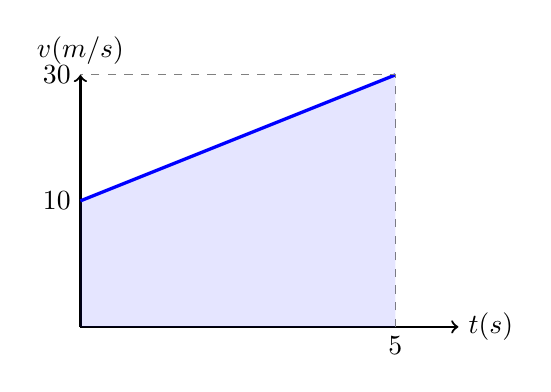
\begin{tikzpicture}[scale=0.8]
            \draw[->,thick] (0,0) -- (6,0) node[right] {$t(s)$};
            \draw[->,thick] (0,0) -- (0,4) node[above] {$v(m/s)$};
            \draw[blue, very thick] (0,2) -- (5,4);
            \draw[dashed, gray] (5,0) node[below, black] {$5$} -- (5,4) -- (0,4) node[left, black] {$30$};
            \draw (0,2) node[left, black] {$10$};
            \fill[blue, opacity=0.1] (0,0) -- (0,2) -- (5,4) -- (5,0) -- cycle;
        \end{tikzpicture}
        \vspace{0.5em}
        \begin{minipage}{0.38\textwidth}
            \captionsetup{type=figure, name=Gráfico, hypcap=false, justification=centering}
            \captionof{figure}{Velocidade escalar de um móvel em função do tempo.}
        \end{minipage}
    \end{minipage}

    \item (Criação Gráfica) Um veículo parte do repouso com aceleração constante de $3$ m/s$^2$ durante $4$ s. Em seguida, mantém a velocidade constante por $2$ s. Esboce o gráfico $v \times t$ para esse intervalo total de $6$ s.

    \item (Criação de Gráfico) Esboce o gráfico da posição pelo tempo ($s \times t$) para um móvel que parte da origem ($s_0=0$) com $v_0=0$ e aceleração $a = 2$ m/s$^2$, para o intervalo de $0$ a $3$ s.

    % --- Nível Médio/Difícil: Aplicações de Fórmulas ---
    \item (Velocidade Média) Um veículo em MRUV aumenta sua velocidade de $15$ m/s para $25$ m/s em um percurso de $200$ m. Qual foi o tempo gasto para realizar esse deslocamento? (Dica: use a média aritmética das velocidades).

    \item Um objeto parte do repouso e descreve um MRUV com aceleração constante de $2$ m/s$^2$. Determine a sua velocidade e a sua posição após $10$ segundos, considerando a posição inicial $s_0 = 0$.

    \item Um móvel parte da posição $s_0 = 20$ m com velocidade inicial $v_0 = -10$ m/s e aceleração constante $a = 4$ m/s$^2$. Determine o instante em que ele passa pela origem das posições ($s = 0$).

    \item Um avião, ao pousar, toca a pista com uma velocidade de $70$ m/s. Sabendo que ele para após percorrer $700$ m em MRUV, determine o valor da aceleração escalar média imposta pelos freios.

    % --- Nível Difícil: Problemas Complexos ---
    \item Um carro está a uma velocidade de $108$ km/h quando o piloto pisa no freio, aplicando uma desaceleração constante de $5$ m/s$^2$. Qual a distância percorrida pelo carro até parar? (Lembre-se de converter a unidade de velocidade).

    \item Um projétil atravessa uma tábua de $10$ cm de espessura. Ele entra na tábua com $400$ m/s e sai com $300$ m/s. Qual o módulo da aceleração média sofrida pelo projétil durante a travessia?

    \item Um trem de $100$ m de comprimento atravessa um túnel de $200$ m. Ele entra no túnel com velocidade de $10$ m/s e sua frente sai dele com velocidade de $20$ m/s. Calcule a aceleração do trem e o tempo gasto para que ele saia \textbf{completamente} do túnel.
\end{enumerate}

%================================
\section{Problemas:}

\begin{enumerate}
    % --- Problema 1: Encontro de Móveis (MRU vs MRUV) ---
    \item Um motorista de aplicativo parado em um semáforo (repouso) parte com uma aceleração constante de $2$ m/s$^2$ no exato instante em que um caminhão o ultrapassa com uma velocidade constante de $14$ m/s. 
    \begin{enumerate}
        \item Após quanto tempo o motorista alcançará o caminhão?
        \item Qual será a velocidade do carro no instante do encontro?
    \end{enumerate}

    % --- Problema 2: Tempo de Reação e Frenagem ---
    \item Um condutor atento dirige seu veículo a $72$ km/h em uma via retilínea. De repente, ele vê um obstáculo e pisa no freio. Sabendo que o tempo de reação do motorista (tempo entre ver o perigo e acionar o freio) é de $0,6$ s e que os freios aplicam uma desaceleração de $5$ m/s$^2$, determine a distância total percorrida desde o instante em que ele vê o obstáculo até a parada total.

    % --- Problema 3: Perseguição com Acelerações Diferentes ---
    \item Dois ciclistas, $A$ e $B$, partem simultaneamente de um mesmo ponto. O ciclista $A$ parte com velocidade inicial de $2$ m/s e aceleração de $1$ m/s$^2$. O ciclista $B$ parte com velocidade inicial de $8$ m/s, mas com uma aceleração de apenas $0,2$ m/s$^2$. Determine a distância percorrida por ambos até que o ciclista $A$ consiga ultrapassar o ciclista $B$.

    % --- Problema 4: Analise de Gráfico por Partes ---
    \item Um trem de metrô parte de uma estação $X$, acelera uniformemente a $1,2$ m/s$^2$ durante $10$ s, mantém a velocidade constante por $30$ s e, em seguida, freia uniformemente com aceleração de $-2$ m/s$^2$ até parar na estação $Y$. 
    \begin{enumerate}
        \item Qual a velocidade máxima atingida pelo trem?
        \item Qual a distância total entre as estações $X$ e $Y$?
    \end{enumerate}

    % --- Problema 5: Ultrapassagem e Comprimento do Veículo ---
    \item Uma carreta de $25$ m de comprimento move-se com velocidade constante de $54$ km/h. Um automóvel, que está logo atrás da carreta, inicia uma ultrapassagem acelerando a $2$ m/s$^2$. Sabendo que o automóvel tem $5$ m de comprimento e que a ultrapassagem termina quando a traseira do carro passa a frente da carreta, calcule:
    \begin{enumerate}
        \item O tempo total de ultrapassagem.
        \item A distância percorrida pelo automóvel durante esse processo.
    \end{enumerate}
\end{enumerate}